\documentclass[border=12pt]{standalone}
% shared preamble for all schematics/diagrams
\usepackage[siunitx, RPvoltages, european resistors]{circuitikz}
\usepackage{tikz}
\usetikzlibrary{arrows.meta,positioning,calc,shapes.geometric,fit,backgrounds,decorations.pathreplacing}
\usepackage[scaled=0.92]{helvet}
\renewcommand{\familydefault}{\sfdefault}
\usepackage{xcolor}
\usepackage{amsmath}
\usepackage{ifthen}
\definecolor{ink}{HTML}{1F2328}
\definecolor{muted}{HTML}{6B6A66}
\definecolor{c1}{HTML}{2A78D6}
\definecolor{c2}{HTML}{EB6834}
\definecolor{c3}{HTML}{1BAF7A}
\definecolor{c4}{HTML}{6250D6}
\definecolor{fill1}{HTML}{EAF2FC}
\definecolor{fill2}{HTML}{FDEEE7}
\definecolor{fill3}{HTML}{E6F6EF}
\definecolor{fill4}{HTML}{EFEDFB}
\definecolor{hv}{HTML}{C62828}
\ctikzset{bipoles/thickness=1.2, monopoles/ground/thickness=1.2}
\tikzset{every picture/.style={line width=0.7pt, color=ink}}

\begin{document}
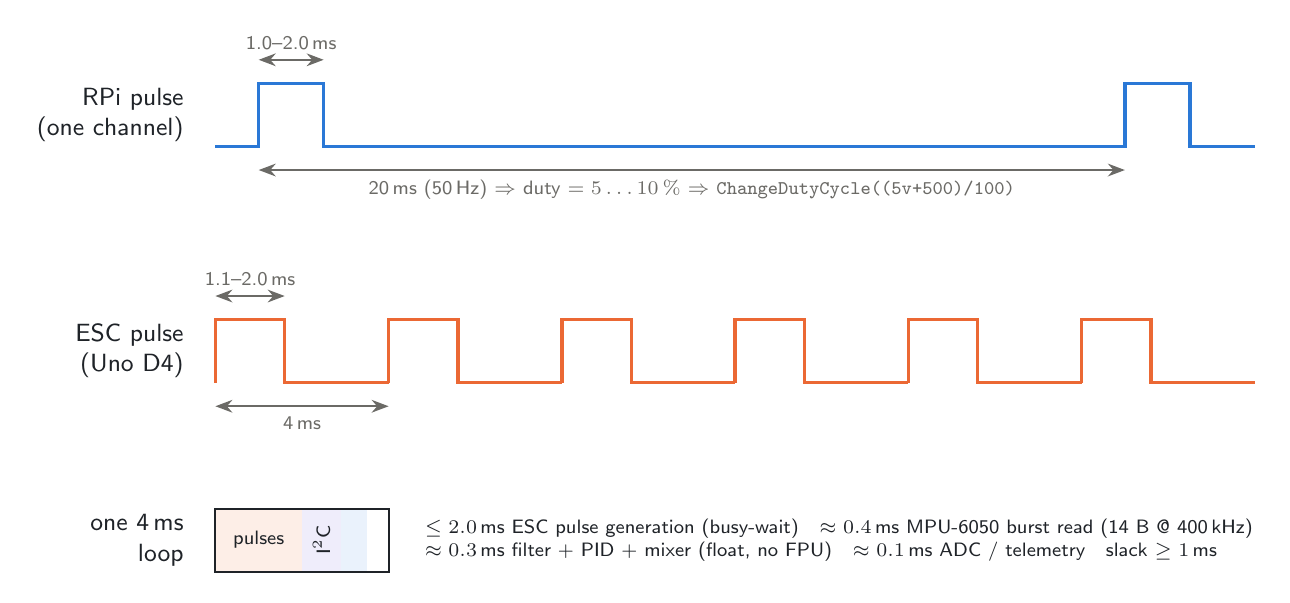
\begin{tikzpicture}[x=0.55cm, y=1cm, w/.style={line width=1.2pt}]
% RPi 50 Hz
\node[anchor=east, font=\small, align=right] at (-0.5,4.4) {RPi pulse\\(one channel)};
\draw[w, c1] (0,4) -- (1,4) -- (1,4.8) -- (2.5,4.8) -- (2.5,4) -- (21,4) -- (21,4.8) -- (22.5,4.8) -- (22.5,4) -- (24,4);
\draw[{Stealth}-{Stealth}, muted] (1,5.1) -- (2.5,5.1) node[midway, above, font=\scriptsize] {1.0--2.0\,ms};
\draw[{Stealth}-{Stealth}, muted] (1,3.7) -- (21,3.7) node[midway, below, font=\scriptsize] {20\,ms (50\,Hz) $\Rightarrow$ duty $= 5\ldots10\,\%$ $\Rightarrow$ \texttt{ChangeDutyCycle((5v+500)/100)}};
% ESC 250 Hz
\node[anchor=east, font=\small, align=right] at (-0.5,1.4) {ESC pulse\\(Uno D4)};
\foreach \s in {0,4,8,12,16,20} {
  \draw[w, c2] (\s,1) -- (\s,1.8) -- (\s+1.6,1.8) -- (\s+1.6,1) -- (\s+4,1);
}
\draw[{Stealth}-{Stealth}, muted] (0,0.7) -- (4,0.7) node[midway, below, font=\scriptsize] {4\,ms};
\draw[{Stealth}-{Stealth}, muted] (0,2.1) -- (1.6,2.1) node[midway, above, font=\scriptsize] {1.1--2.0\,ms};
% loop budget
\node[anchor=east, font=\small, align=right] at (-0.5,-1.0) {one 4\,ms\\loop};
\fill[fill2] (0,-1.4) rectangle (2,-0.6); \node[font=\scriptsize] at (1,-1.0) {pulses};
\fill[fill4] (2,-1.4) rectangle (2.9,-0.6); \node[font=\scriptsize, rotate=90] at (2.45,-1.0) {I$^2$C};
\fill[fill1] (2.9,-1.4) rectangle (3.5,-0.6);
\fill[white] (3.5,-1.4) rectangle (4,-0.6);
\draw (0,-1.4) rectangle (4,-0.6);
\node[font=\scriptsize, align=left, anchor=west] at (4.6,-1.0) {
$\leq 2.0$\,ms ESC pulse generation (busy-wait)\quad 
$\approx 0.4$\,ms MPU-6050 burst read (14 B @ 400\,kHz)\\
$\approx 0.3$\,ms filter + PID + mixer (float, no FPU)\quad $\approx 0.1$\,ms ADC / telemetry\quad slack $\geq 1$\,ms};
\end{tikzpicture}
\end{document}
